
\section{Γιατί το χρησιμοποιούμε;}
    \paragraph{}
    Είναι πλέον κοινά παραδεκτό ότι ένας αναγνώστης αποσπάται από το περιεχόμενο που διαβάζει, όταν εξετάζει τη διαμόρφωση
    μίας σελίδας.

    \begin{figure}[h!]
        \centering
        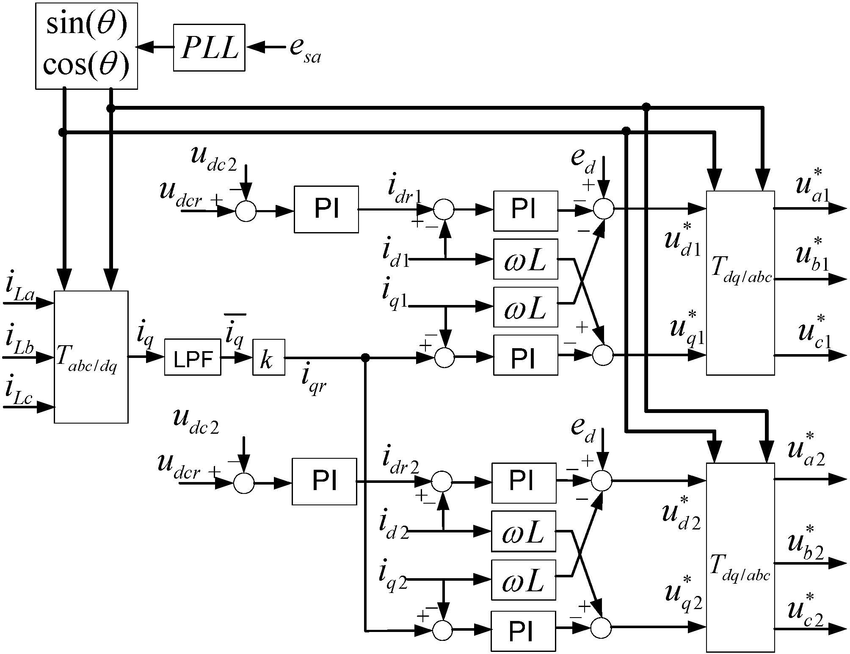
\includegraphics[scale=0.3]{assets/figures/figure_1.png}
        \caption{Αυτός είναι ο υπότιτλος του σχήματος}
        \label{fig:figure of something}
    \end{figure}
    
    \subsection{Αυτό είναι υποενότητα}
    \paragraph{}
    Η ουσία της χρήσης του Lorem Ipsum είναι ότι έχει λίγο-πολύ μία ομαλή κατανομή γραμμάτων, αντίθετα με το
    να βάλει κανείς κείμενο όπως 'Εδώ θα μπει κείμενο, εδώ θα μπει κείμενο', κάνοντάς το να φαίνεται σαν κανονικό κείμενο.
    Δες σχήμα \ref{fig:figure of something}

    \subsection{Αυτό είναι υποενότητα}
    \paragraph{}
    Πολλά λογισμικά πακέτα ηλεκτρονικής σελιδοποίησης και επεξεργαστές ιστότοπων πλέον χρησιμοποιούν το Lorem Ipsum σαν
    προκαθορισμένο δείγμα κειμένου, και η αναζήτησ για τις λέξεις 'lorem ipsum' στο διαδίκτυο θα αποκαλύψει πολλά web site
    που βρίσκονται στο στάδιο της δημιουργίας. Διάφορες εκδοχές έχουν προκύψει με το πέρασμα των χρόνων, άλλες φορές κατά
    λάθος, άλλες φορές σκόπιμα (με σκοπό το χιούμορ και άλλα συναφή).

    \begin{table}[h!]
        \centering
        \caption{Fisher's Iris data}
        \label{tab:table1}
        % This is to resize the table to fit the page
        \resizebox{\linewidth}{!}{%
        % With l,c,r you define the alignment of each column
        \begin{tabular}{l||c|c|c|c|r}
            Dataset Order & Sepal Length & Sepal Width & Petal Length & Petal Length & Species\\
            \hline
            1 &	5.1 & 3.5 & 1.4 & 0.2 & I. setosa\\
            2 &	4.9 & 3.0 & 1.4 & 0.2 & I. setosa\\
            3 &	4.7 & 3.2 & 1.3 & 0.2 & I. setosa\\
            4 &	4.6 & 3.1 & 1.5 & 0.2 & I. setosa\\
        \end{tabular}
        }
    \end{table}

% It creates a nice aesthetic to start a new chapter/section in a new page
\newpage
